%%%%%%%%%%%%%%%%%%%%%%%%%%%%%%%%%
%
%       EXERCÍCIO
%
%%%%%%%%%%%%%%%%%%%%%%%%%%%%%%%%%

\ifdefstring{\atividade}{prova}{%
    \ifdefstring{\modo}{objetivo}{%
        \renewcommand{\valorquestao}{\ValorQObj\ ponto}
    }{%
        \renewcommand{\valorquestao}{\ValorQDisc\ pontos}
    }%
}%

\begin{exercicioBanco}[\valorquestao]
Em uma pesquisa, obteve‑se o gráfico abaixo, que indica o crescimento de uma cultura de bactérias no decorrer de \(6\) meses.

\begin{center}
    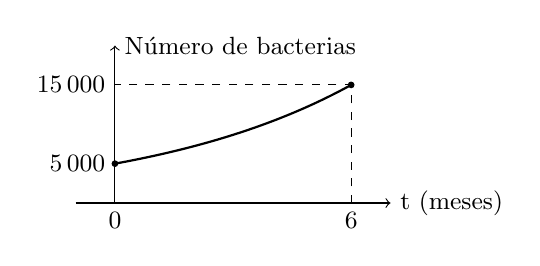
\begin{tikzpicture}[scale=0.5]
        % Eixos
        \draw[->] (-1,0) -- (7,0) node[right] {\small \shortstack{t (meses)}};
        \draw[->] (0,0) -- (0,4) node[right] {\small Número de bacterias};
        
        % Pontos de referência
        \draw[dashed] (6,0) -- (6,3) -- (0,3);
        
        % Pontos e marcações
        \filldraw (0,1) circle (2pt);
        \filldraw (6,3) circle (2pt);
        \node[left] at (0,1) {\small \(5\,000\)};
        \node[left] at (0,3) {\small \(15\,000\)};
        \node[below] at (0,0) {\small \(0\)};
        \node[below] at (6,0) {\small \(6\)};

        % Curva da parábola com vértice em (15,13.5)
        \draw[domain=0:6, smooth, samples=100, thick] 
            plot (\x, {(3)^(\x/6)});
    \end{tikzpicture}
\end{center}

Admitindo a lei de formação da função que representa essa situação como \(f(t) = ka^{t}\), determine os valores de \(k\) e de \(a\).

% Define as alternativas
\newcommand{\alternativas}{%
    \begin{center}
        \begin{tabularx}{\textwidth}{XXX}
            (a) \(k = 1\) e \(a = 2\). &
            (b) \(k = 5\,000\) e \(a = \sqrt[6]{3}\). &
            (c) \(k = 15\,000\) e \(a = \sqrt{3}\). \\[5pt]
            (d) \(k = \dfrac{1}{2}\) e \(a = 3\). &
            (e) \(k = \sqrt{2}\) e \(a = \dfrac{1}{2}\).
        \end{tabularx}
    \end{center}
}

% Define a resposta correta
\newcommand{\resposta}{B}

% Lógica condicional para exibição
\ifdefstring{\atividade}{lista}{%
    \alternativas
    \vspace{0.5em}
    
    \noindent\textbf{Resposta:} letra \textbf{\resposta}.
}{%
    \ifdefstring{\modo}{objetivo}{%
        \alternativas
    }{%
        % modo = discursiva → não mostra alternativas
    }
}
\end{exercicioBanco}

